\section {Online Sketch Maintenance}\label{sec:online}
In the offline scenario, all the events about every subject are assumed 
to be available at the time of sketch computation. 
In contrast, in the online scenario,
events arrive incrementally. 
Given an arrival event, our objective is to keep the sketch 
for each subject up-to-date. Since the event arrival speed could be very high, such step has to been done very efficiently.  

Similar to the offline scenario, we maintain a $WI$ to keep 
track of the $p$ best event windows (candidate themes) 
for all the possible window lengths.
To handle a newly arrived event $e_s(t)$, a naive solution would generate
all the event windows containing $e_s(t)$, (i.e. $W_s(t,w'), w'\in(1,t]$). For each
event window, $WI$ is then updated accordingly. 
Afterwards, Algorithm~\ref{algo:greedy} needs to be
invoked to re-compute the sketches. 
However, there are $t$ associated event windows for each new event $e_s(t)$. 
Examining all of them is too expensive to support real-time responses. 
Moreover, Algorithm~\ref{algo:greedy} runs in $O(k|\mathbb{N}_s|)$ time for each affected subject, which imposes further performance challenge. 

To achieve instant sketch update, we propose two techniques - \emph{window pruning} and \emph{sketch maintenance}. Window pruning tries to reduce the number of windows evaluated in generating candidate themes. After obtaining the candidate themes, we need to update the sketches affected. As we shall see later, given a candidate theme $N_s(t,w)$, not only the sketch for subject $s$ but also the sketches for other subjects could be affected. Although in the offline scenario we provided a solution with a $(1-1/e)$ approximation, to maintain sketches with the same approximation ratio is difficult in the online scenario~\cite{Alonerbuch2003The,Awerbuch1996Making}. Instead, we propose a $1/8$-approximation solution for sketch maintenance which only takes $O(k)$ time to perform the sketch update.

\begin{algorithm}[h]
\caption{Online Query}\label{algo:online_overview}
\begin{algorithmic}[1]
\Require $e_s(t) \gets $ arrival event
\State $WI()$ $p$ best event windows for each window length
\State $\beta()$ smallest score in $WI$ for each window length
\For{$w \in 1,...,t $}
\If{$W_s(t,w)$ can be added to $WI(w)$}
\State update $\beta(w)$, $J_s(w)$, compute $N_s(t,w)$ 
\State UpdateSketches($N_s(t,w)$)
\EndIf
\State $P_s(w) = \frac{w}{w+1}W_s(t,w).\overline{v}+\frac{t-w}{w+1}J_s(t-w)$
\State \bf{break} if $P_s(w)\leq \max\{\beta(w')|w < w' \leq t\}$
\EndFor
\end{algorithmic}
\end{algorithm}

Before we present \emph{window pruning} and \emph{sketch maintenance}, 
Algorithm~\ref{algo:online_overview} 
demonstrates the overview of our online solution against a new event $e_s(t)$. 
We iteratively examine 
event windows which contain $e_s(t)$ (i.e.,$W_s(t,w)$ in Line 4). 
We then update the sketches which are affected by inserting $W_s(t,w)$ into $WI$ (Lines 5-6). Before continuing to examine the next event window $w$,
we compute the maximum score (i.e., $P_s(w)$) of all event windows which have not been evaluated. If $P_s(w)$ is smaller than all $\beta(w'), w' \in (w,t]$, we can safely stop the process since no further event window could cause any sketches to change.

\subsection{Online Window Pruning}
Since there are $t$ event windows associated with each new event $e_s(t)$, 
we wish to avoid enumerating all the possible cases. 
We achieve the window pruning by leveraging the online-window bound $P_s(w)$, which
is the upper bound score among event windows with length greater than $w$. 
The value of $P_s(w)$ is stated as in the following theorem:

\begin{theorem}[Online-Window Bound]
\label{thm:online_bound}
Let $W_s(t,1)$,...,$W_s(t,w)$ be the $w$ event windows computed in Algorithm~\ref{algo:online_overview} containing event $e_s(t)$. Let $P_s(w)$ be:
\begin{equation}
	P_s(w) = \frac{w}{w+1}W_s(t,w).\overline{v}+ min\{\frac{t-w}{w+1}J_s(t-w), \frac{t-w}{t}J_s(1) \}
\end{equation}
Where $J_s(\cdot)$ is the visiting-window bound.  Then $P_s(w)$ is the online-window bound, i.e.,$P_s(w) \geq \max\{W_s(t,x).\overline{v}| w < x \leq t \}$.
\end{theorem}
\begin{proof}
First, $\forall x \in (w,t]$, we have: 
\begin{align*}
W_s(t,x).\overline{v} &= \frac{w*W_s(t,w).\overline{v} + (x-w)*W_s(t-w,x-w).\overline{v}}{x} \\
%& = \frac{w*W_s(t,w).\overline{v}}{x} + \frac{(x-w)*W_s(t-w,x-w).\overline{v}}{x} \\
& \leq \frac{w*W_s(t,w).\overline{v}}{w+1} + \frac{(x-w)*W_s(t-w,x-w).\overline{v}}{x}
\end{align*}
Note that $J_s(x-w) \geq W_s(t-w, x-w).\overline{v}$, and $yJ_s(y)$ monotonically increases wrt. $y$.
It follows that $(x-w)W_s(t-w,x-w).\overline{v}/{x} \leq (x-w)J_s(x-w)/{x} \leq (t-w)J_s(t-w)/(w+1)$.

On the other hand, $J_s(1)\geq W_s(\cdot,y).\overline{v}$, for any $y$. Therefore,
$(x-w)W_s(t-w,x-w).\overline{v}/{x} \leq (x-w)J_s(1)/x \leq (t-w)J_s(1)/t$.
Combining the above deductions, it follows that:
\begin{equation*}
\hspace{-4mm}\frac{(x-w)W_s(t-w,x-w).\overline{v}}{x} \leq min\{\frac{t-w}{w+1}J_s(t-w), \frac{t-w}{t}J_s(1) \}
\end{equation*}
which naturally leads to Theorem~\ref{thm:online_bound}. 
\end{proof}

When $w$ is small, $\frac{t-w}{w+1}J_s(t-w)$ is too loose as $\frac{t-w}{w+1}$ is large. However, we can leverage $\frac{t-w}{t}J_s(1)$ to obtain a better bound. As $w$ increases, $\frac{t-w}{w+1}J_s(t-w)$ eventually becomes smaller than $\frac{t-w}{t}J_s(1)$. Thus, we leverage $\frac{t-w}{w+1}J_s(t-w)$ to perform efficient pruning. 

%Using the same logic, we can derive bounds for other aggregate functions; these are listed in Section~\ref{sec:discussion}.

\subsection{Sketch Maintenance}
\label{subsec:sketch_main}
Once we obtain an event window $W_s(t,w)$ which causes changes in the $WI(w)$, two kinds of sketch maintenances may occur. The first is 
to update the sketch for subject $s$, which we refer to as \emph{active-update}. The second is to update the sketches for other subjects. This happens when some of their candidate themes' ranks  become worse due to $W_s(t,w)$. We refer to this case as \emph{passive-update}. If these updates are not properly handled, sketches maintained for those subjects are not able to obtain an approximate ratio on their qualities. We demonstrate these updates in the following example.

\begin{figure}
	\centering
    \begin{subfigure}[b]{0.45\textwidth}
        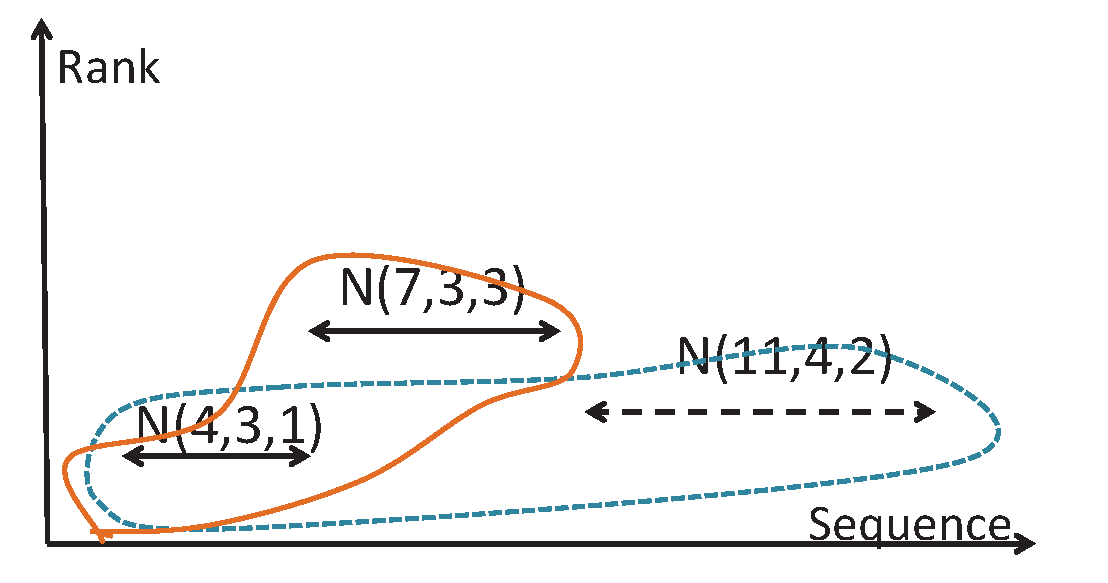
\includegraphics[width=\textwidth]{chapter4/charts/active_update.eps}
        \caption{Active update of new candidate theme $N(11,4)$}
%        \label{fig:active_update}
    \end{subfigure}
    \begin{subfigure}[b]{0.45\textwidth}
        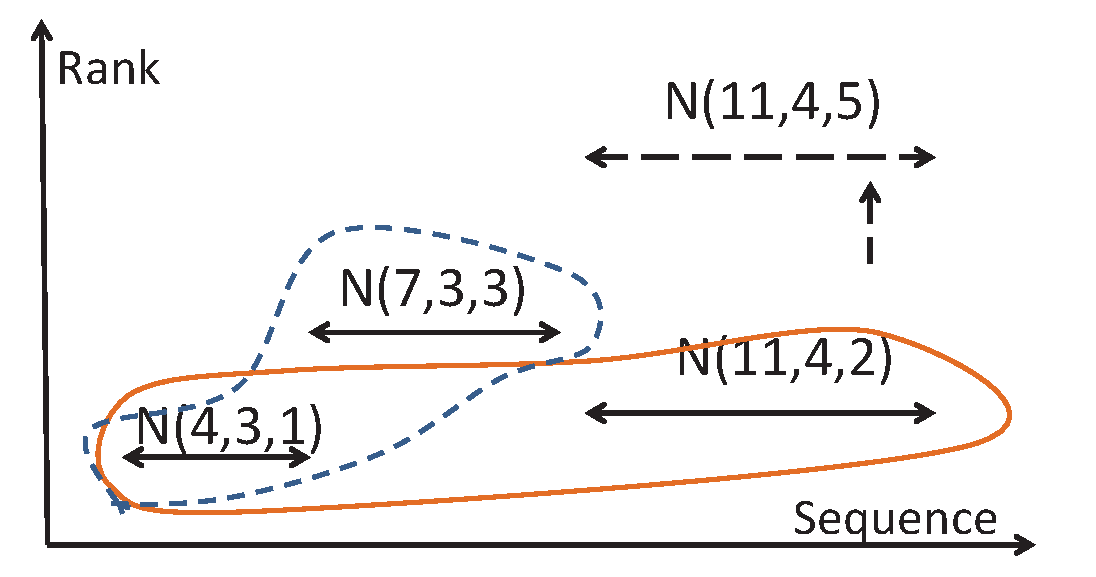
\includegraphics[width=\textwidth]{chapter4/charts/passive_update.eps}
        \caption{Passive update due to existing candidate theme $N(11,4)$ }
%        \label{fig:passive_update}
    \end{subfigure}
    \caption{The illustration of active updates and passive updates, the solid circle represent the original
    sketch, the dotted circle represent the updated sketch.}
    \label{fig:sketch_maintenance}
\end{figure}


\begin{example}
Suppose $k = 2$ and we maintain a $2$-Sketch for each subject. As shown in Fig.~\ref{fig:sketch_maintenance}(a), 
when the candidate theme $N(11,4)$ is generated, the maintained sketch is no longer the best. This is because replacing 
$N(7,3)$ would generate a better sketch. This process is referred as \emph{active update}.
In Fig.~\ref{fig:sketch_maintenance}(b), $N(11,4)$ is pushed up due to the arrival of the event about another subject; as a result, the quality of the sketch drops. We name this process as \emph{passive update}. If passive update is not handled, the rank of $N(11,4)$ may continue to be pushing up and may eventually be greater than $p$, making the entire sketch invalid. Nevertheless, it is evident that when $N(11,4)$ degrades, replacing it with $N(7,3)$ would
result in a sketch with better quality. 
\end{example}

A naive approach to handle online update is to run Algorithm~\ref{algo:greedy} for subjects whose sketches are affected.
This maintains a $(1-1/e)$ approximation ratio but incurs high computational overheads. In order to support efficient updates, we make a trade-off between the quality of the sketch and the update efficiency by providing a $1/8$ approximation solution with only $O(k)$ candidate themes being accessed for each affecting subject. 

%Unlike the naive approach which checks every candidate theme to update a sketch, 
%only $2k$ candidate themes are required for each subject in our approach. 
In particular, we maintain two sets $S_1$ and $S_2$ each of size $k$. 
$S_1$ maintains the $k$ best candidate themes which collectively cover the most
events whereas $S_2$ maintains $k$ candidate themes with best ranks. When performing an active update for a candidate theme $N_s(t,w)$, we check if $N_s(t,w)$ could replace any candidates in $S_1$ to generate a better cover meanwhile we select the new $k$ best ranked candidate themes into $S_2$. After $S_1$ is updated, we perform the greedy selection among candidate themes in $S_1 \cup S_2$.
During a passive update, $S_1$ is not affected. We simply update $S_2$ to be the new $k$ best ranked candidate themes. 
After that, the new sketch is obtained by performing a greedy selection on $S_1 \cup S_2$. Algorithm~\ref{algo:online_update} summarizes both the active and passive update. 
%
%Let scoring function $C(S)$ be the cardinality of sequences covered by all elements in $S$, $R_i$ be the
%all news candidates of object $i$, then our algorithm works as follows: 
\begin{algorithm}
\caption{UpdateSketches}\label{algo:online_update}
\begin{algorithmic} [1]
\Require $N_s(t,w)$
\State \textbf{Active update for the subject $s$}
\State $S_1$:  $k$ candidate themes with best cover
\State $S_2$:  $k$ candidate themes with best ranks 
\State $N^* \gets \argmax_{N \in S_1}C(S_1 \cup N_s(t,w) \setminus N)$
\If{$C(S_1) < C(S_1 \cup N_s(t,w) \setminus N^*)$}
\State $S_1 \gets S_1 \cup N_s(t,w) \setminus N^*$
\EndIf
\State $S_2 \gets$ new $k$ best candidates for rank scores 
\State $greedy(S_1 \cup S_2 )$
\\\hrulefill
\State \textbf{Passive update for an affecting subject $s'$}
\State $S_2 \gets$ new $k$ best candidates for rank score $s'$ 
\State $S \gets greedy(S_1 \cup S_2)$
\end{algorithmic}
\end{algorithm}
  
%\begin{algorithm}
%\caption{Passive Update for Subject $s$}
%\begin{algorithmic} [1]
%\end{algorithmic}
%\label{algo:online_passive_update}
%\end{algorithm}

Given our sketch update strategies, we are now ready to prove the approximation ratio for the maintained sketches. 

\begin{theorem}[Approximation Ratio for Sketch Update]
\label{thm:online_quality}
Each sketch maintained by Algorithms~\ref{algo:online_overview}
achieves an at least $1/8$ approximation to optimal solution.
\end{theorem}

\begin{proof}
First, we observe that $S_2$ always keep the candidates with optimal ranks. 
Second, we note that $S_1$ maintains the candidates with 1/4 optimality as shown in~\cite{Saha2009On}.

Let $OPT_C$ be the optimal solution for $k$ best covering of $s$'s events; Let $C()$ be the number of events a set of candidate theme covers. Similarly, let $OPT_R$ be the optimal solution for $k$ best ranked candidate themes of $s$; Let $R()$ be the 
summation of ranks of all members in a candidate theme set. Let $S^*_s$ be the optimal sketch of subject $s$. Intuitively, we have the following: 
\begin{equation*} 
g'(S^*_s) \leq \eta_1 C(OPT_C) + \eta_2 R(OPT_R)
\end{equation*}
Since $C(S_1) \geq 1/4 C(OPT_C)$ and $R(S_2) = R(OPT_R)$, we have the following:
\begin{equation*}
\begin{split}
\eta_1 C(S_1) + \eta_2 R(S_2) & \geq 1/4 * \eta_1 C(OPT_C) + \eta_2 R(OPT_R) \\
& \geq 1/4 g'(S^*_s)
\end{split}
\end{equation*}
, which implies $\max\{\eta_1 C(S_1), \eta_2 R(S_2)\} \geq 1/8 g( S^*_s)$. 
As $g'(S_1) \geq \eta_1 C(S_1)$ and $g'(S_2) > \eta_2 R(S_2)$, it leads to:
\begin{equation*}
\max\{g'(S_1), g'(S_2)\} > 1/8  g'(S^*_s)
\end{equation*}
Let $SK_s$ be one of the sketch maintained by Algorithms~\ref{algo:online_update},
since the greedy algorithm is run on $S_1 \cup S_2$, 
$g'(SK_s) \geq max(g'(S_1), g'(S_2)) \geq 1/8 g'(S^*_s)$.
As a result, our algorithm always ensures a 1/8 approximation ratio for each sketch.
\end{proof}

%We model the news selection problem as follows: Given a event
%$e$, let $C$ denote the news candidates derived from $e$. Each news
%candidate is of the form $\langle sid, w, t, r\rangle$, where $sid$ is the
%identifier of subject, $w$ is the
%length of this news candidate, $t$ is the end time this candidate and $r$
%is the rank of this news candidate w.r.t other news candidates with 
%similar window size. 
%
%Let $R(sid, T)$ be the set of news that has been reported of subject $sid$ prior to
%the time sequence $T$, i.e., $R(sid,T)={n| n.sid = sid, n.t < T}$. When no ambiguity, 
%we use $R(T)$ for short.
%In order to maintain the quality of the news reported for a subject, we 
%wish to fulfill the following two criteria:
%\begin{enumerate}
%\item the news candidates in $R(T)$ needs to cover the most events in the subject's history
%\item the ranks of the news in $R(T)$ needs to be as low as possible
%\end{enumerate}
%
%The first criteria tends to provide the comprehensive news which covers the subject's
%past history, the second criteria tends to select the most quality news out of the news candidate.
%
%Therefore, given a set of news, we define a evaluation function as follows:
%\begin{equation}
%	F(X) =  \Sigma_{n \in X}(n.w * n.r)
%\end{equation}
%
%In order to consider both criteria, we insert \emph{unit news candidate} of form $u(t_i)=\langle sid,1,t_i,R\rangle$
%,where $R$ is the maximum rank that considered to be meaningful. For $R(T)$, we insert $T$ unit
%news candidates into it, so that our problem is defined to be a set cover: Given $R(T) = {S_1,S_2,...,S_k}$ where 
%each $S_i$ is a (unit) news candidate. Consider a ground set $G = \{1,...,T\}$. Our objective is to find a set $X \subseteq R$ 
%such that $\cup_{x_i \in X} [x_i.t-w, x_i.t] \supseteq G$ and $F(X)$ is minimized.

%The online version of the problem is that, given two sets $R(T-1)$ and $C(T)$ where $R(T-1)$ is the reported
%news and $C(T)$ is the online derived news candidates. Our objective is to find a subset $C' \subseteq C$ such that
%$\cup_{x_i \in (R \cup C')}[x_i.t-w, x_i.t] \supseteq (G \cup T+1)$ and $F(R \cup C')$ is minimized.
%
%It is easy to see that, the online version of the problem can be used for new events reporting, while
%the offline version of the problem can be used for history analysis of subjects.


%\subsubsection{Optimal Method for Offline Problem}
%The offline method is clearly a weighted vertex cover problem which is known to be NP-hard.
%For this problem, the optimal solution can be achieved via dynamic programming. Let $M[i][X]$
%be the \emph{optimal} value for using sets $S_1,S_2,...,S_i$ in set $R$ covering sets $X$, 
%we have the following relationship:
%\begin{equation}
%M[i][X] = min\{M[i-1][X-S_i] + S_i.r, M[i-1][X]\}
%\end{equation}
%
%Based on the equation, the optimal dynamic programming algorithm takes $O(k\times 2 ^{t})$ space
%and time. Although by some careful design, the space is able to reduce to $O(2^{t})$, both the 
%space and time complexity are not feasible for relatively large number of news detection. 
%
%We tackle the high complexity by first providing a branch-and-bound search for dynamic programming.
%Our main observation is that there exists dominance relationship between news events.

%\section{View Based Query Processing}
%In this section, we propose a view based query processing strategy to 
%timely process each arriving event. The notations used in the remaining
%of the paper is shown in Table~\ref{tbl:notations}.
%
%
%
%In our framework, processing a new 
%event $e=(id,V,s)$ consists of three phases. First, the event window $W_1$,...,$W_{s}$
%are derived. Second, for each event window $W_w$, its corresponding news candidate is
%formed by $N_w=\langle id, w, f_a(W_w), r \rangle$. Third, each $N_w$ is assessed by
%the scoring function $S$ and filtered by the threshold $\eta$.
%
%The main bottleneck of the processing is on second step where each $W_w$ needs to find 
%its rank among \textbf{all} other window events with the same size. If there are $s$ subjects
%in the application history, with each subjects has $m$ events, there are $O(ms)$ comparisons
%required to find $f_a(W_w)$'s rank.   
%
%
%Continuous Aggregation Detection for a new event $e=(o,a,v,t)$ entails 
%two phases. The first phase is to generate all possible event windows containing $e$. This results in $|t|$ new event windows. The second phase is 
%to verify that any of these $t$ new event windows are belong to the corresponding top-$k$ list. 
%
%To efficiently accomplish the second phase, the \emph{Top-$k$ Event Window Index} $H$ is necessary. Basically, for each window size $w$, $H_w$ maintains the top-$k$ lists of window event of size $w$. Given the set of existing events, $H$ can be built in off-line.
%
%A brute-force approach is thus as follows: \textbf{off-line phase}: For each $w$, generate the all possible event window of size $w$. Create $H_w$ with the top-$k$ event windows of size $w$. \textbf{on-line phase}: For newly arrived event $e$, for each $w$, compute the event window of size $w$ containing $e$.  Check for each $w$, report $e$ and $w$ if the event window is in $H_w$. 
%
%A simple analysis reveals the inefficiencies in the brute-force approach. In off-line phase, suppose there are $n$ objects, each with $w$ events, there are $\Theta(nw^2)$ event windows. Then computing the top-$k$ events is at least $\Theta(log(k)nw^2)$. In online phase, generating all $w$ event windows takes $\Theta(w)$ while checking for top-$k$ existence takes $\Theta(log(k))$. So the total complexity for a single event query is $\Theta(log(k)w)$.
%
%The inefficiencies with brute-force approach lies in: in off-line phase, it compute \textbf{every} window sizes for \textbf{every} object to generate the index. In on-line phase, it checks for event window of \textbf{every} size to report the full results. We thus devise several optimization to reduce the overhead. In the following sections, we will describe our techniques in two aspects: the index construction and query processing.

